\documentclass{article}

% set font encoding for PDFLaTeX or XeLaTeX
\usepackage{graphicx}
\usepackage{ifxetex}
\usepackage{hyperref}

\ifxetex
  \usepackage{fontspec}
\else
  \usepackage[T1]{fontenc}
  \usepackage[utf8]{inputenc}
  \usepackage{lmodern}
\fi
\title{Actividad 3}
\author{Fisica Computacional 1\\
Corral Valdez Jesus Giovanni\\
Departamento de Física\\
Universidad de Sonora}
\date{}
% Enable SageTeX to run SageMath code right inside this LaTeX file.
% documentation: http://mirrors.ctan.org/macros/latex/contrib/sagetex/sagetexpackage.pdf
% \usepackage{sagetex}

\begin{document}
\maketitle
\clearpage
\section{Introducción}
Durante esta segunda actividad, se analizara datos parecidos a los de la Actividad 1, pero ahora son numeros recolectados por la propia Universidad de Sonora en el manglar de El Sargento\\
\begin{figure}[h]
  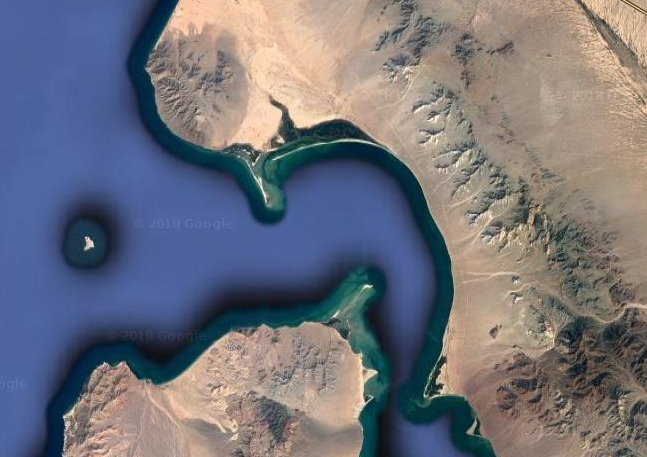
\includegraphics[width=\linewidth]{Tiburon.png}
\end{figure}
\\
También se probara la herramienta de Plotly para los gráficos necesarios\\
\begin{figure}[h]
  
\includegraphics[width=\linewidth]{3-00.png}
\end{figure}

\clearpage
\section{Desarrollo}
1.Se importó nuestra nueva herramienta y demás librerías que se utilizarán.\\
\begin{figure}[h]
  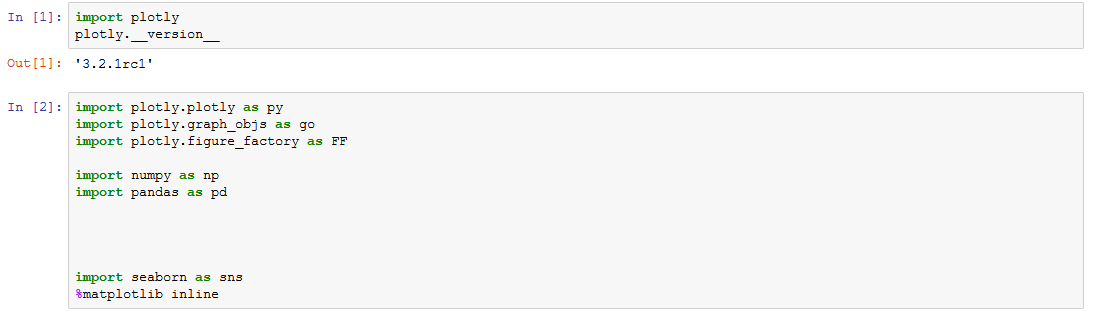
\includegraphics[width=\linewidth]{3-01.png}
\end{figure}
\\
2.Sargento cuenta con dos sensores, el cual uno lo llamaremos "Canal" y el otro "Estación". Al importar sus csv de datos, le asignaremos nombre a sus columnas.\\
\begin{figure}[h]
  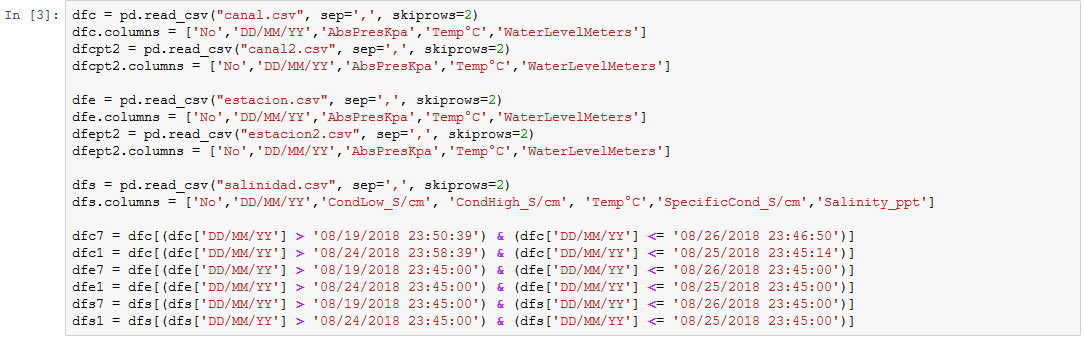
\includegraphics[width=\linewidth]{3-02.png}
\end{figure}
Se dividió cada una de estas listas en dos periodos, de un día y una semana para hacer mas sencilla su comparación y además se agregó datos sobre la salinidad de la zona de la Estación. \\
\clearpage
3.Nuestras primera gráficas en Plotly serán una sencilla comparación del nivel del agua de la zona de la estación y de la zona del canal, respecto a un día y una semana.\\
\begin{figure}[h]
  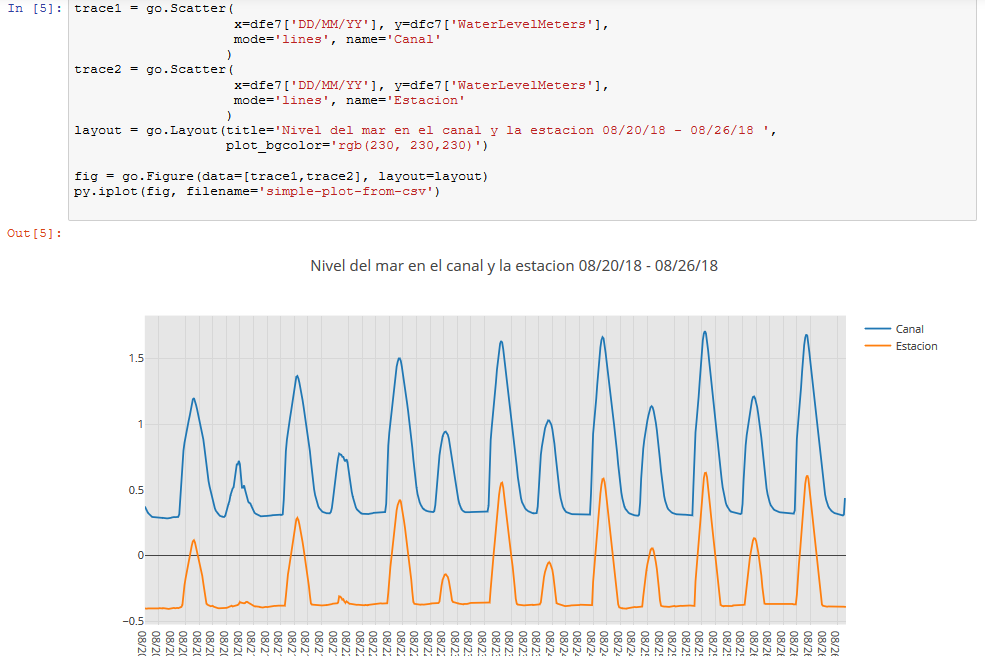
\includegraphics[width=\linewidth]{3-03.png}
\end{figure}
\begin{figure}[h]
  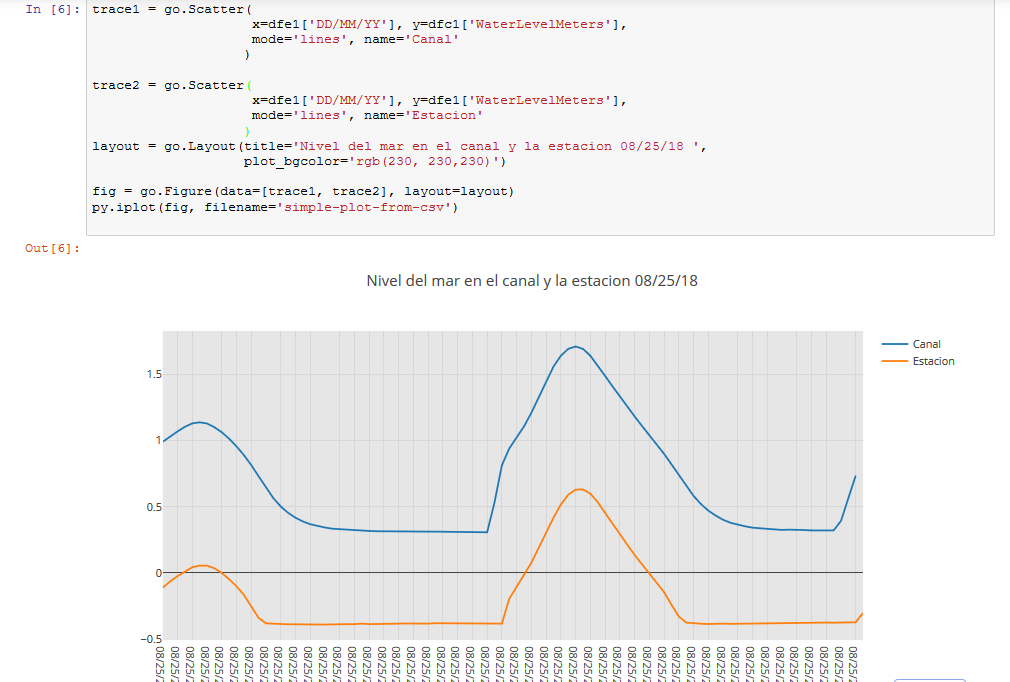
\includegraphics[width=\linewidth]{3-04.png}
\end{figure}

\clearpage
4.Contamos con datos de la salinidad en la estación así que la graficaremos respecto a al nivel del mar en el mismo tiempo para encontrar si existe alguna relación.\\
\begin{figure}[h]
  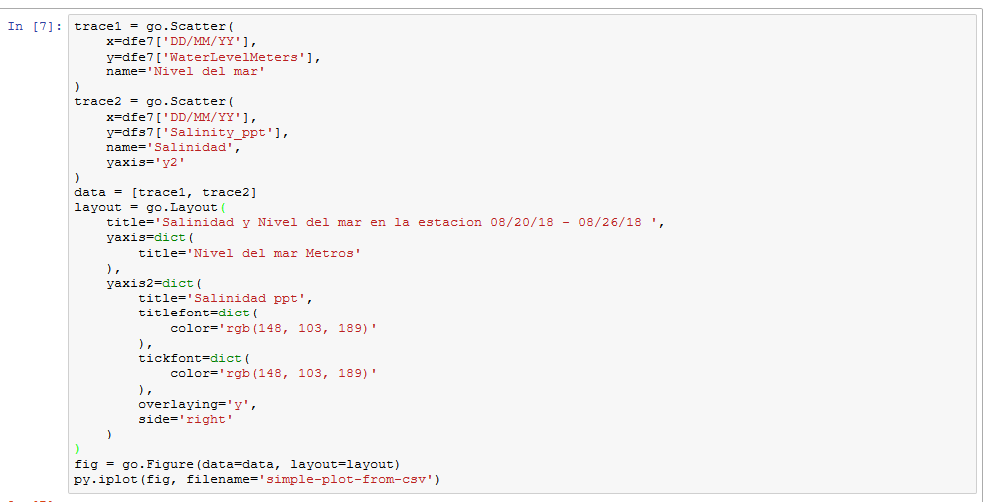
\includegraphics[width=\linewidth]{3-05.png}
\end{figure}
\begin{figure}[h]
  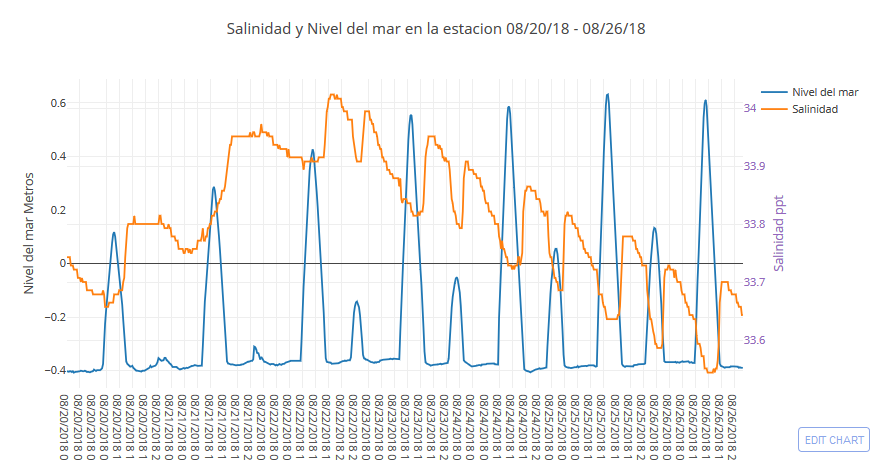
\includegraphics[width=\linewidth]{3-05-2.png}
\end{figure}
\begin{figure}[h]
  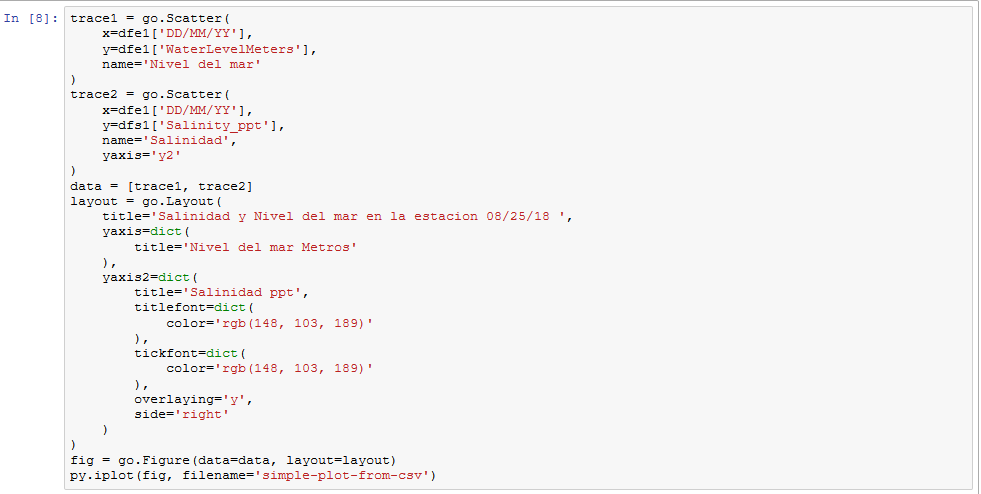
\includegraphics[width=\linewidth]{3-06.png}
\end{figure}
\begin{figure}[h]
  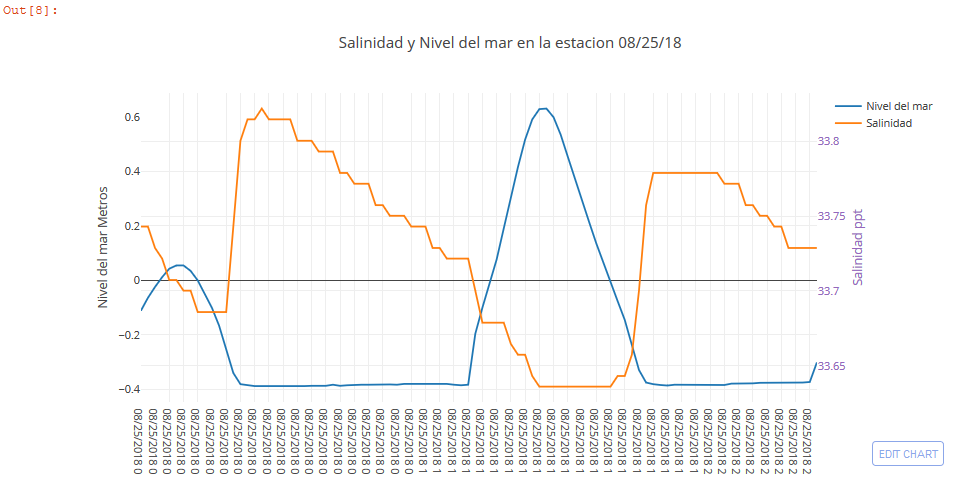
\includegraphics[width=\linewidth]{3-06-2.png}
\end{figure}

\clearpage
5.También se graficaron los datos de la temperatura de la estación.\\
\begin{figure}[h]
  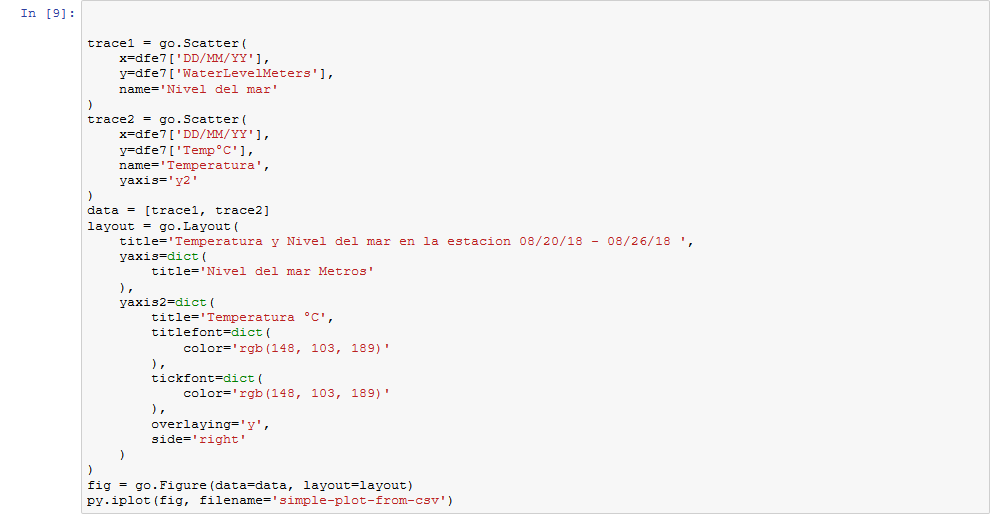
\includegraphics[width=\linewidth]{3-07.png}
\end{figure}

\begin{figure}[h]
  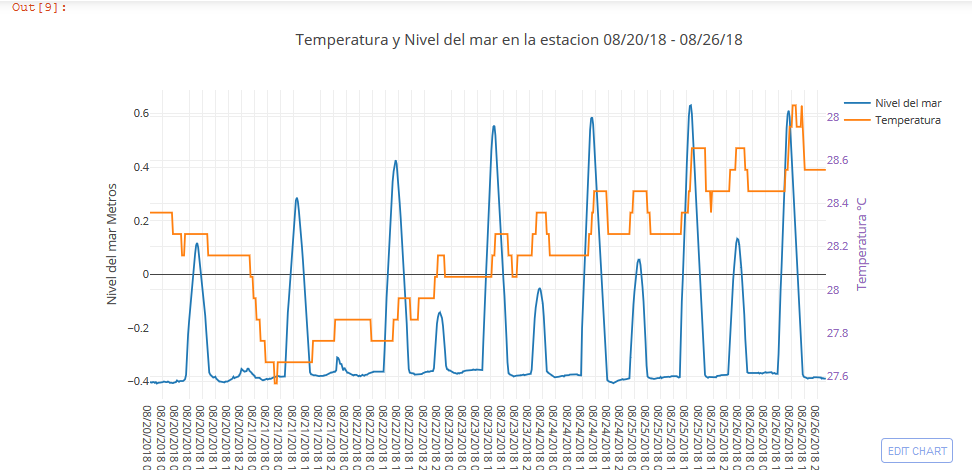
\includegraphics[width=\linewidth]{3-07-2.png}
\end{figure}

\begin{figure}[h]
  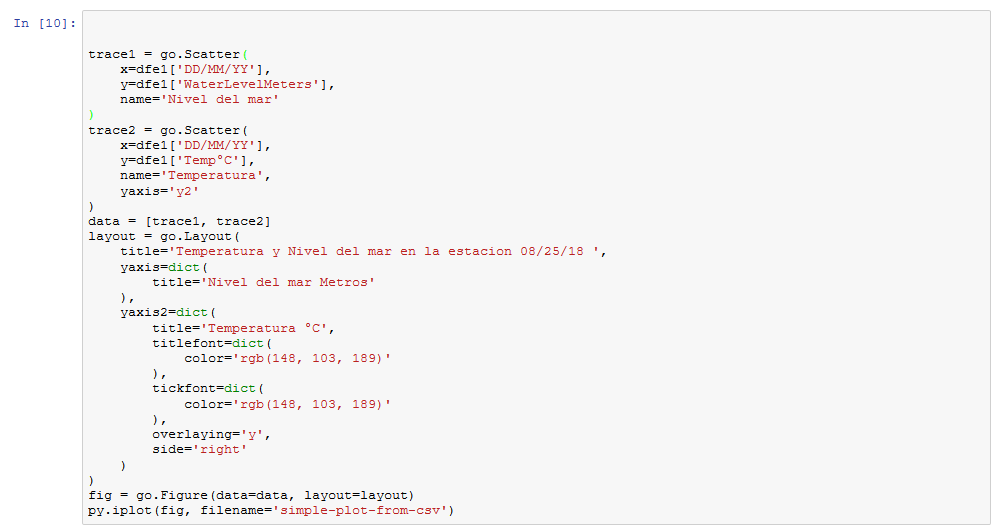
\includegraphics[width=\linewidth]{3-08.png}
\end{figure}
\begin{figure}[h]
  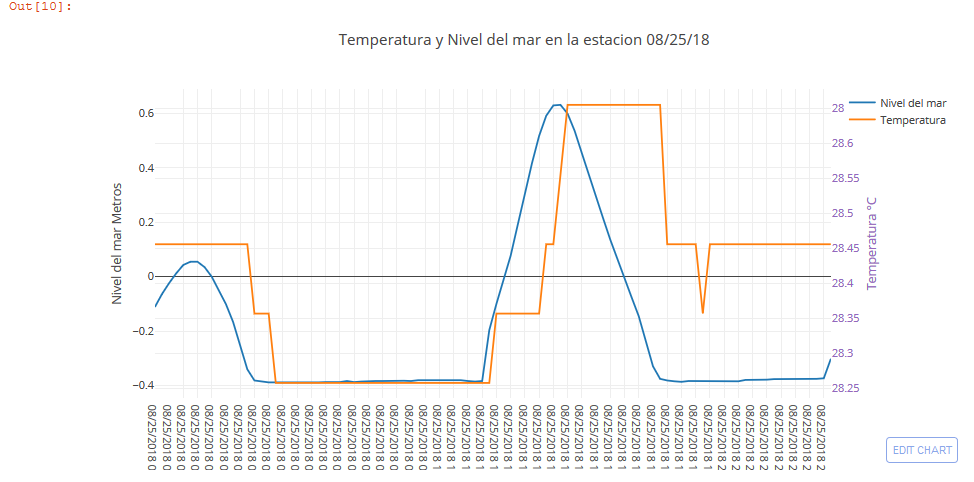
\includegraphics[width=\linewidth]{3-08-2.png}
\end{figure}
\clearpage

6.Y ahora lo mismo con la temperatura del canal.\\
\begin{figure}[h]
  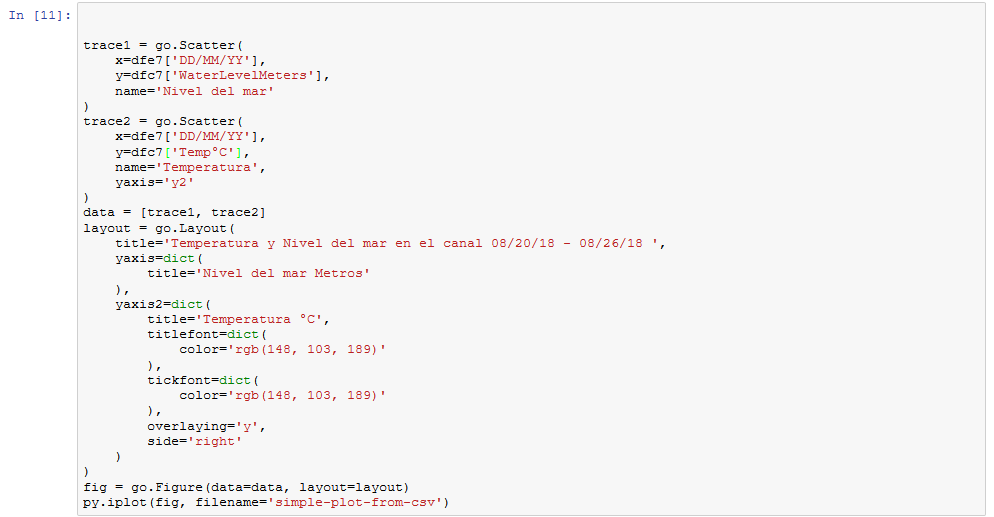
\includegraphics[width=\linewidth]{3-09.png}
\end{figure}
\begin{figure}[h]
  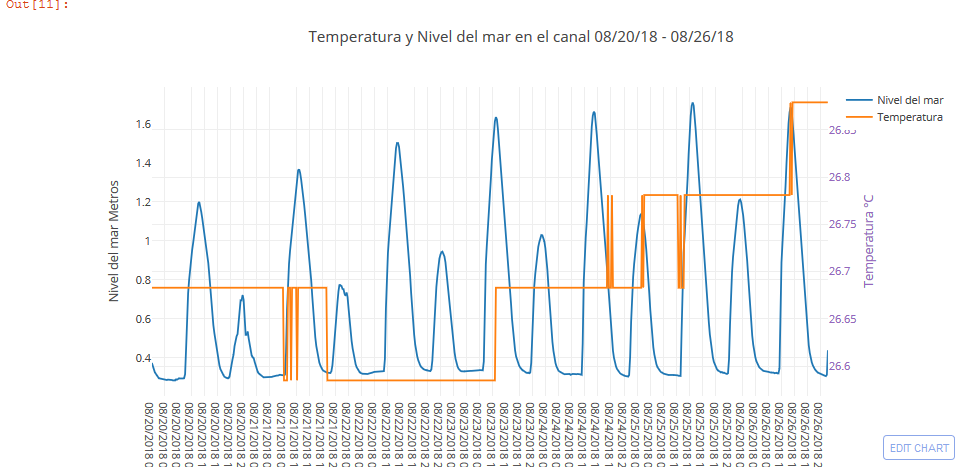
\includegraphics[width=\linewidth]{3-09-2.png}
\end{figure}
\begin{figure}[h]
  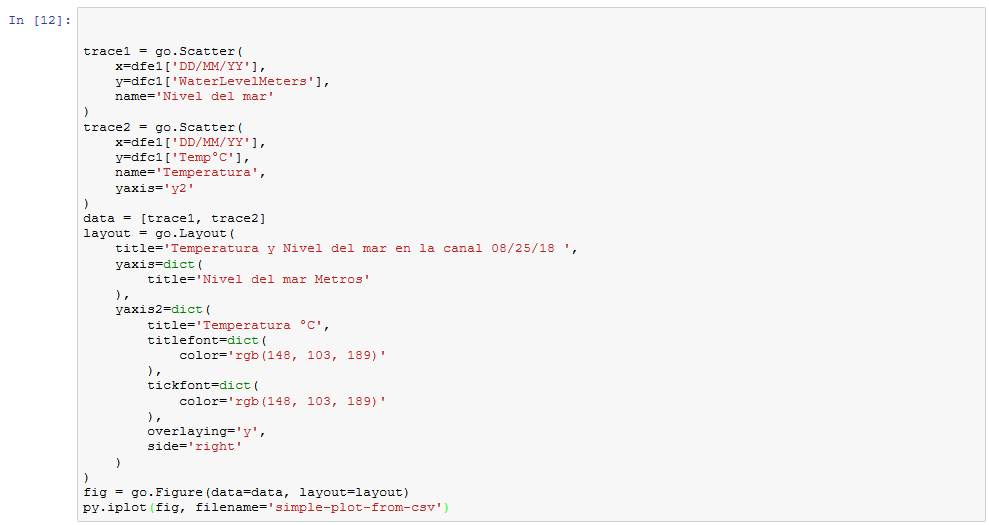
\includegraphics[width=\linewidth]{3-10.png}
\end{figure}
\begin{figure}[h]
  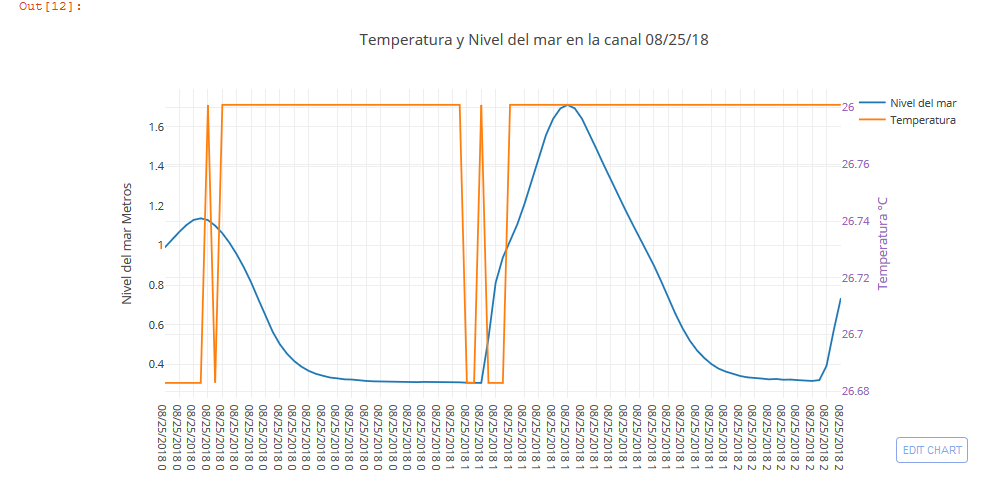
\includegraphics[width=\linewidth]{3-10-2.png}
\end{figure}
\clearpage
7.A veces se puede obviar una correlación con las graficas, pero como nuestro objetivo es saber con mas certeza esto, se realiza una tabla de correlación entre las tablas de datos de la estación.\\
\begin{figure}[h]
  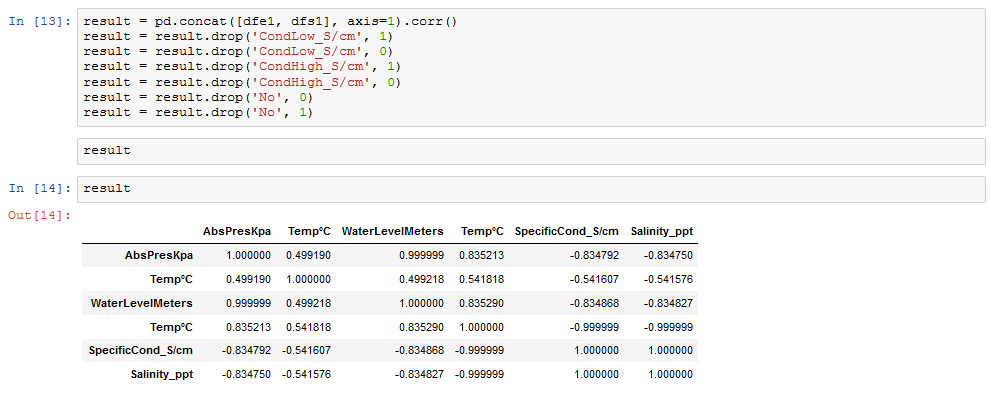
\includegraphics[width=\linewidth]{3-11.png}
\end{figure}
Y con estos datos es posible hacer un mapa de calor y encontrar las correlaciones entre las variables, que durante la actividad nos interesamos por la temperatura y la salinidad respecto al nivel del mar.
\begin{figure}[h]
  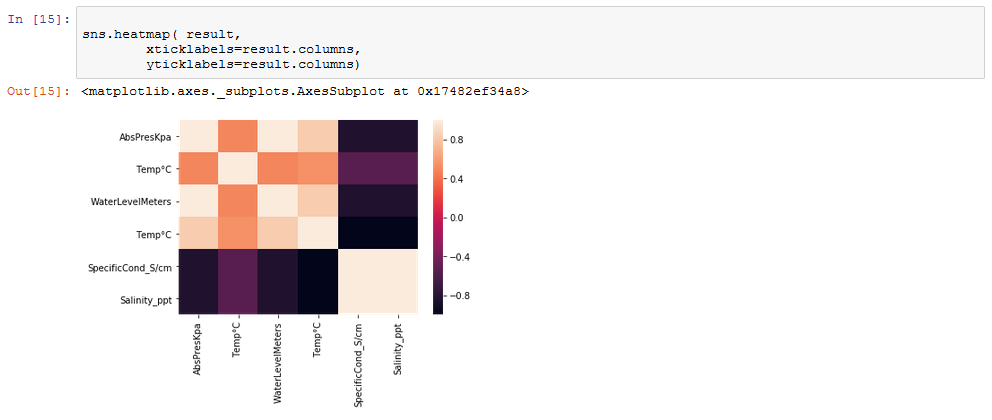
\includegraphics[width=\linewidth]{3-11-2.png}
\end{figure}
\clearpage

\section{Conclusión}
Gracias a Plotly nuestro análisis es mas sencillo por su propiedad de ser interactiva y mucho mas estética que otros graficadores en Python. Respecto a lo que lleva al análisis de datos en esta actividad, podemos encontrar dos relaciones muy importantes en el mapa de calor:\\
Correlación entre nivel del mar y Temperatura = 0.835290.\\
Correlación entre nivel del mar y Salinidad = -0.834827.\\
Y curiosamente la correlación entre Temperatura y Salinidad es casi del -1.00.\\
De estos datos se pueden concluir varias cosas:\\
*La temperatura aumenta cuando sube el nivel del mar, porque entra agua de afuera del manglar que esta caliente por la radiación del sol.\\
*La salinidad disminuye al subir el nivel del mar porque la sal que se habia quedado estancada se mezcla con mas cantidad de agua.




\end{document}
